\documentclass[prb,preprint]{revtex4-2} 
% The line above defines the type of LaTeX document.
% Note that AJP uses the same style as Phys. Rev. B (prb).
\usepackage{amsmath}  % needed for \tfrac, \bmatrix, etc.
\usepackage{amsfonts} % needed for bold Greek, Fraktur, and blackboard bold
\usepackage{graphicx} % needed for figures



%% formatted for IOP
%%\documentclass[12pt]{iopart}

%PLOS guidelines
%https://journals.plos.org/plosone/s/submission-guidelines
% possible editor, Luís A. Nunes Amaral
% ORCID Icon orcid.org/0000-0002-3762-789X
%\pdfminorversion=4

\usepackage{float}
\usepackage{units}
\usepackage{graphicx}
\usepackage{hyperref}

\newcommand{\be}{\begin{equation}}
\newcommand{\ee}{\end{equation}}
\newcommand{\bea}{\begin{eqnarray}}
\newcommand{\eea}{\end{eqnarray}}
\newcommand{\degC}{^{\circ}C}

\begin{document}

\title{Hypothesis creation with fluffy baby chicks} 

\author{Tom Reigstad}
\email{treigstad@cotterschools.org}
\affiliation{Science, Cotter Schools, Winona, MN 55987}

\author{Sara E. Moore}
\email{}
\affiliation{Cotter Elementary School, Winona State University, Winona, MN 55987}


\author{Nathan T. Moore}
\email{nmoore@winona.edu}
\affiliation{Physics, Winona State University, Winona, MN 55987}

\date{\today}

\begin{abstract}
In the spring term it is fun to hatch chickens in a science class. 
Not every egg hatches, and thinking about what variables accurately predict whether an egg will hatch is a useful hypothesis creation opportunity.
As chicken embroys develop, the mass of a chicken egg decreases substantially, and watching this variable over time can be a good opportunity for students to accurately ``predict the future'' and when coupled with candling, revise their predictions based on updated observation. 
\end{abstract}
\maketitle

\section{Introduction}
Living in almost rural Minnesota, for the past several years we have hatched chicken eggs in our elementary, high-school, and college classrooms.  Even at college age, students are excited about hatching and fluffy baby chicks, and the activity is an obvious opportunity to talk about reproduction, anatomy, and (what other standards???).  We use inexpensive foam incubators\cite{incubator_source} with automatic turners, carefully monitor temperature and humidity, and get fresh eggs from people with both backyard hens and roosters, but despite our best efforts, many incubations end up full of ``bummers'' like those shown in figure \ref{incubator}, with hatch rates of about $50--75\%$ success. 

``What went wrong?'' is a common student question at the end of the 3 week long incubation.  The public library books \cite{chicken_ref} and University Extension pages \cite{U_extension} are full of advice and precaution we may have forgotten to take.  Eggs don't all incubate at the same temperature.  Snakes need a temperature of ???, turtles ???, and chickens $37.5\degC$.  
Ducks are normally damp, and duck eggs need to be dabbed with water each day for ducklings to be able to tear the shell membrane open.  
Eggs need to be turned regularly.
oil from hands can fill eggshell pores
antibacterial bloom
eggs collected in February might freeze
fertility drops with a hen's age.
rooster to hen ratio, turkey insemination. 


Instead of, or at least in addition to, going in that discussion with an incubation, we've taken the opportunity to survey student ideas about what factors could be used to predict if a given egg will hatch.  The rest of the paper describes student ideas, and gives details on egg mass, which is probably one of the better ways to track development.  
    
\begin{figure}[h]
\centering
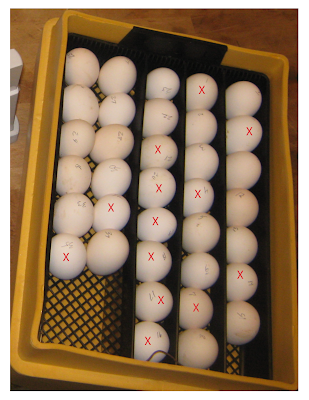
\includegraphics[width=\columnwidth]{did_not_hatch.png}
\caption{
example image, Eggs in the incubator.  Those with a red X did not hatch.
}
\label{incubator}
\end{figure}

\section{Student Ideas}


\section{Egg mass}

\begin{figure}[h]
\centering
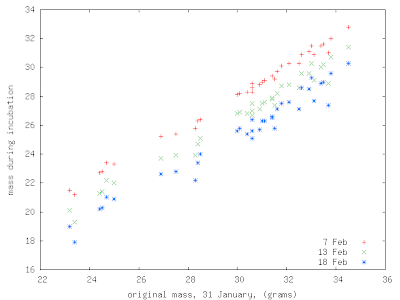
\includegraphics[width=\columnwidth]{egg_mass_over_time.png}
\caption{
example image, For some incubations we have massed each egg over the course of the incubation.  Typically, eggs lose about $15\%$ of their mass over the course of the $21\pm2$ day incubation. In this figure, the horizontal coordinate is an egg's mass when the incubation started.  The vertical coordinate is the mass at a later time.  If an egg lost NO mass, it would lie on the $y=x$ diagonal in this graph.  
}
\label{incubator}
\end{figure}


\section{Conclusion}

\begin{acknowledgments}

\end{acknowledgments}

%\begin{table}
%\centering
%\caption{
%A summary of units and conversions used to create figure \ref{ag_yields} from USDA NASS data.  $1cwt$ is a hundred pounds of potatoes.  
%A bushel, $1bu$, is a volume unit of about 35liters and corresponds to about 60lbs of grain. Calorie content per 100 gram (mass) of food is taken from the USDA's ``Food Data Central'' database. 
%For context, typical serving sizes are included. 
%It isn't clear from any of these resources if lb is pound-force (lbf) or pound-mass (lbm) and so I am treating them as ``grocery store units'' where $1 lbs \approx 453.6 grams$.
%}
%%%\begin{indented}
%%%\item[]\begin{tabular}{@{}llllll}
%\begin{ruledtabular}
%%%\begin{tabular}{@{}llllll}\br
%\begin{tabular}{l l l l l l}
%Crop&per acre unit&production unit&kcals per 100gram & typical portion &FDC ID\\
%%%\mr
%\hline
%Corn & bu/acre & $1bu=56lbs$ & 365 & 1 cup is 166g &170288 \\
%Potatoes & cwt/acre & $1CWT=100lbs$ & 77 & 0.5 cup is 75g & 170026 \\
%Soybeans & bu/acre & $1bu=60lbs$ & 446 & 1 cup is 186g &174270 \\
%Sunflowers & lbs/acre & & 584 & 1 cup is 140g & 170562 \\
%Wheat & bu/acre & $1bu=60lbs$ & 327 &  1 cup is 192g & 168890 \\
%%\br
%\end{tabular}
%\end{ruledtabular}
%%%\end{indented}
%\label{conversions}
%\end{table}
%

\section*{References}
\begin{thebibliography}{99}

\bibitem{incubator_source}
Most recently we've used Model 4250 from \url{https://www.farminnovators.com/poultry.html#incubators}, but the analog incubators are fine too.  Eggs must be regularly turned for embroyos to develop properly.  

\bibitem{chicken ref}

\bibitem{U_extension}

\bibitem{Energy_textbook}
Jack J. Kraushaar, Robert A. Ristinen, and Jeffrey T. Brack,
\textit{Energy and the Environment}, 
4th edition
(Wiley, 2022).

\bibitem{meat_sweats}
%https://www.bonappetit.com/story/meat-sweats
P. Trayhurn,
``Thermogenesis,''
in \textit{Encyclopedia of Food Sciences and Nutrition. 2nd ed.},
edited by Benjamin Caballero 
(Academic Press, 2003), pp. 5762-7.
%ISBN 9780122270550,
%https://doi.org/10.1016/B0-12-227055-X/01188-3.
%(https://www.sciencedirect.com/science/article/pii/B012227055X011883)


\end{thebibliography}


\end{document}
